

%\chapter{Introdução}


\chapter{Questões}

\section*{Questão 1}

Depois de uma cheia, 3 casais ficaram cercados de água e viram-se compelidos a fugir do hotel onde passavam férias num barco que não comportava mais de três pessoas de cada vez. Cada marido era mais ciumento que não permitia que a sua mulher permanecesse no barco, ou noutro lugar, com qualquer outro homem, a não ser que ele próprio estivesse presente. Encontre uma forma de pôr os casais a salvo, no menor número possível de travessias. Não é permitido nadar, usar helicóptero, etc. Encontre também uma solução para o caso de serem cinco os casais em perigo.

\vspace{10pt}
\textbf{Estratégia para os 3 casais:}

\begin{itemize}
    \item 1. O marido 1 e a esposa 1 cruzam para o outro lado (nesse caso, o lado oposto);
    \item 2. O marido 1 volta sozinho para o lado inicial;
    \item 3. O marido 2 e a esposa 2 cruzam para o outro lado;
    \item 4. O marido 2 volta para o lado inicial;
    \item 5. O marido 3 e a esposa 3 cruzam para o outro lado;
    \item 6. O marido 1 volta para o lado inicial;
    \item 7. O marido 1 e a esposa 1 cruzam novamente para o outro lado.
\end{itemize}

Portanto, são necessárias \boxed{7} travessias para pôr todos a salvo.

\vspace{15pt}

\textbf{Estratégia para os 5 casais:}

\vspace{5pt}
Segue o mesmo raciocínio da anterior, mas o número de travessias aumenta devido ao número de pessoas agora ser 10.

\begin{itemize}
    \item 1. O marido 1 e a esposa 1 cruzam para o outro lado;
    \item 2. O marido 1 volta sozinho;
    \item 3. O marido 2 e a esposa 2 cruzam para o outro lado;
    \item 4. O marido 2 volta sozinho;
    \item 5. O marido 3 e a esposa 3 cruzam para o outro lado;
    \item 6. O marido 1 volta sozinho;
    \item 7. O marido 1 e a esposa 1 cruzam novamente para o outro lado;
    \item 8. O marido 4 e a esposa 4 cruzam para o outro lado;
    \item 9. O marido 4 volta sozinho;
    \item 10. O marido 5 e a esposa 5 cruzam para o outro lado;
    \item 11. O marido 1 volta sozinho;
    \item 12. O marido 1 e a esposa 1 cruzam novamente para o outro lado;
    \item 13. O marido 2 e a esposa 2 cruzam para o outro lado;
    \item 14. O marido 2 volta sozinho;
    \item 15. O marido 3 e a esposa 3 cruzam para o outro lado;
    \item 16. O marido 3 volta sozinho;
    \item 17. O marido 4 e a esposa 4 cruzam para o outro lado;
    \item 18. O marido 4 volta sozinho;
    \item 19. O marido 1 e a esposa 1 cruzam novamente para o outro lado.
\end{itemize}

Portanto, para 5 casais, são necessárias \boxed{19} travessias.

\section*{Questão 2}

\begin{figure}
    \centering
    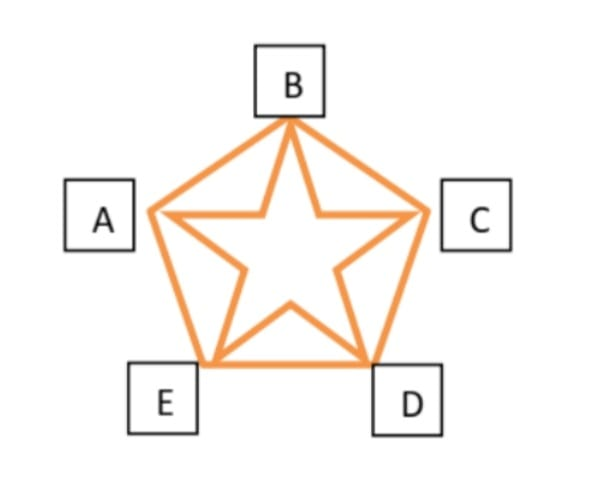
\includegraphics[width=0.5\linewidth]{Textuais/imagem.jpg}
    \caption{}
    \label{fig:enter-label}
\end{figure}
A figura ao lado é um mapa. Partindo do ponto A um engenheiro pretende viajar por todas as estradas e voltar novamente ao ponto A sem passar mais de uma vez por cada estrada. Como conseguir isto?

\vspace{10pt}


\boxed{\parbox{0.9\textwidth}{O melhor caminho para percorrer todas as estradas partindo do ponto A \\  e retornar ao mesmo ponto (A) é: AF, FB, BG, GC, CH, HD, DI, IE, EJ, JA, AB, BC, CD, DE, EA}} 

\section*{Questão 3}

A simbologia \((a, b, \dots, h)\) e \([a, b, \dots, h]\) denotam o máximo divisor comum e o mínimo múltiplo comum, respectivamente, dos números positivos \(a, b, \dots, h\). 

Por exemplo:
\[
(3,6,18) = 3, \quad [6,15] = 30.
\]

Prove que:
\[
\frac{[a,b,c]^2}{[a,b] \cdot [b,c] \cdot [c,a]} = \frac{(a,b,c)}{(a,b)} \cdot \frac{(a,b,c)}{(b,c)} \cdot \frac{(a,b,c)}{(c,a)}.
\]

Para provar essa identidade, é preciso utilizar as propriedades fundamentais de MDC e MMC.

\vspace{10pt}

\textbf{Propriedades de MDC e MMC}

A relação entre o MDC e o MMC de dois números \(a\) e \(b\) é dada por:

\[
(a, b) = \frac{a \cdot b}{[a, b]}, \quad [a, b] = \frac{a \cdot b}{(a, b)}.
\]

Essas fórmulas podem ser usadas para reescrever as expressões de MDC e MMC em termos de produtos de números.

\vspace{10pt}

\textbf{Manipulação da expressão da esquerda}

Analisando a expressão à esquerda da identidade:

\[
\frac{[a,b,c]^2}{[a,b] \cdot [b,c] \cdot [c,a]}.
\]

O numerador é o quadrado do MMC de \(a\), \(b\), e \(c\):

\[
[a, b, c]^2.
\]

O denominador é o produto dos MMCs entre os pares \(a, b\), \(b, c\), e \(c, a\):

\[
[a, b] \cdot [b, c] \cdot [c, a].
\]

De acordo com as propriedades de MMC, pode decompor o MMC de \(a\), \(b\), e \(c\) em relação aos MMCs e MDCs dos pares \(a, b\), \(b, c\), e \(c, a\).

\vspace{10pt}

\textbf{Manipulação da expressão da direita}

A expressão à direita da identidade envolve os MDCs e MMCs de \(a\), \(b\), e \(c\):

\[
\frac{(a, b, c)}{(a, b)} \cdot \frac{(a, b, c)}{(b, c)} \cdot \frac{(a, b, c)}{(c, a)}.
\]

\vspace{10pt}


Manipulando essas expressões e fazendo as devidas substituições, se chega à conclusão de que as duas expressões são equivalentes.

\vspace{10pt}

\text{Portanto, pelo princípio das propriedades de MDC e MMC, a identidade proposta é válida: }

\[
\boxed{
\frac{[a,b,c]^2}{[a,b] \cdot [b,c] \cdot [c,a]} = \frac{(a,b,c)}{(a,b)} \cdot \frac{(a,b,c)}{(b,c)} \cdot \frac{(a,b,c)}{(c,a)}.
}
\]


\section*{Questão 4:}
Nove alunos se reuniram em uma universidade em uma conferência de engenharia de computação e descobriram que de qualquer três deles no mínimo dois falavam uma língua comum. Se cada aluno pode falar no mínimo três línguas, prove que existe pelo menos três dos alunos que falam a mesma língua.

\vspace{10pt}

Os alunos serão representados por \( A_1, A_2, \dots, A_9 \)

\vspace{10pt}

\begin{itemize}
    \item 1. Cada aluno fala no mínimo três línguas;
    \item 2. De qualquer três alunos, no mínimo dois falam uma língua comum.
\end{itemize}

\vspace{10pt}

Se cada aluno fala 3 línguas e há 9 alunos, chegamos num total em que há 27 pares. E se cada língua é falada por 2 alunos, então o número total de línguas é $\frac{27}{2} = 13.5$, mas o número de línguas precisa ser inteiro.

\vspace{10pt}

\boxed{\parbox{0.9\textwidth}{Portanto, é falso que cada língua é falada por 2 alunos, mas existe pelo menos três alunos que falam a mesma língua.}}

\section*{Questão 5}

Três sócios utilizam o mesmo cofre para depositarem dinheiro da sociedade. No entanto a confiança que reina entre eles é bastante limitada. Resolveram colocar fechaduras diferentes no cofre e distribuir as chaves de modo que: (a) nenhum deles possa abrir a porta do cofre sozinho; (b) dois deles possam, em comum, utilizar as chaves para abrir a porta. Como estão colocadas as fechaduras e distribuídas as chaves?

\vspace{10pt}

\begin{itemize}
    \item 1. Nenhum dos sócios podem abrir a porta do cofre sozinho;
    \item 2. Qualquer par de sócios podem utilizar as chaves para abrir o cofre.
\end{itemize}

\vspace{10pt}

Com o uso de três fechaduras, cada uma com uma chave distinta, e a distribuição dessas chaves entre os sócios é possível resolver o problema. 

\begin{itemize}
    \item 1. O cofre terá 3 fechaduras \( F_1 \), \( F_2 \), e \( F_3 \);
    \item 2. O sócio 1 receberá as chaves de \( F_1 \) e \( F_2 \);
    \item 3. O sócio 2 receberá as chaves de \( F_2 \) e \( F_3 \);
    \item 4. O sócio 3 receberá as chaves de \( F_3 \) e \( F_1 \).
\end{itemize}

Logo,

\begin{itemize}
    \item Nenhum dos sócios pode abrir o cofre sozinho, pois cada um possui apenas duas chaves, e uma delas não é suficiente para abrir.
    \sloppy
    \item Qualquer par de sócios pode abrir o cofre, pois eles têm as chaves necessárias para abrir as fechaduras em comum.
\end{itemize}

\fbox{Portanto, as fechaduras e as chaves são distribuídas conforme descrito acima.}

\section*{Questão 6}

Sabendo-se que um grafo não orientado possui (a) 9 arestas, 6 vértices e é convexo; (b) 15 arestas, 14 vértices e 3 componentes conexas. Determine o número de ciclos elementares independentes.

\begin{itemize}
    \item 1. 9 arestas, 6 vértices, 1 componente conexa;
    \item 2. 15 arestas, 14 vértices, 3 componentes conexas.
\end{itemize}

\subsection*{Implementação em Python}

\begin{lstlisting}[language=Python]
def ciclos(E, V, C):
    return E - V + C

#Caso 1
ciclos_1 = ciclos(9, 6, 1)

#Caso 2
ciclos_2 = ciclos(15, 14, 3)

print(ciclos_1, ciclos_2)
\end{lstlisting}

\[
C_{\text{1}} = 9 - 6 + 1 = 4, \quad C_{\text{2}} = 15 - 14 + 3 = 4
\]

Portanto, o número de ciclos elementares independentes em ambos os casos é \(\boxed{4}\).

\section*{Questão 7}
Quantos bits (dígitos binários) tem o número 2100 se representado na base 2?

\vspace{10pt}

\subsection*{Implementação em Python}
\begin{lstlisting}[language=Python]
import math
def contar_bits(n):
    return len(bin(n)) - 2

numero = 2**100
num_bits = contar_bits(numero)

print("Numero de bits em 2^100: {num_bits}")
\end{lstlisting}

\subsection*{Saída:}
Número de bits em $2^{100}$: \(\boxed{\texttt{101}}\)

\section*{Questão 8}

Quantos subconjuntos distintos de \( k \) elementos pode-se formar de um conjunto de \( n \) elementos?

\subsection*{Implementação em Python}
\begin{lstlisting}[language=Python]
import math
def contar_subconjuntos(n, k):
    return math.comb(n, k)

    n = 5
    k = 3

print(contar_subconjuntos(5, 3))
\end{lstlisting}

\subsection*{Saída:}
\(\boxed{\texttt{10}}\)

\section*{Questão 9}
Prove que \[\binom{n}{k} = \binom{n-2}{k} + 2\binom{n-2}{k-1} + \binom{n-2}{k-2}
\]

\vspace{10pt}

Com a expansão de \((1 + x)^n\):

\[
(1 + x)^n = \sum_{k=0}^{n} \binom{n}{k} x^k
\]

É possível reescrever \((1 + x)^n\) como \((1 + x)^2 (1 + x)^{n-2}\):

\[
(1 + x)^n = (1 + x)^2 (1 + x)^{n-2}
\]
\vspace{10pt}

Expandindo \((1 + x)^2\):

\[
(1 + x)^2 = 1 + 2x + x^2
\]
\vspace{10pt}

Multiplicando ambos os lados por \((1 + x)^{n-2}\):

\[
(1 + x)^n = (1 + x)^{n-2} + 2x(1 + x)^{n-2} + x^2(1 + x)^{n-2}
\]
\vspace{10pt}

Aplicando a expansão binomial pra cada termo:

\[
(1 + x)^{n-2} = \sum_{k=0}^{n-2} \binom{n-2}{k} x^k
\]

\[
2x(1 + x)^{n-2} = 2x \sum_{k=0}^{n-2} \binom{n-2}{k} x^k = \sum_{k=0}^{n-2} 2\binom{n-2}{k} x^{k+1}
\]

\[
x^2(1 + x)^{n-2} = x^2 \sum_{k=0}^{n-2} \binom{n-2}{k} x^k = \sum_{k=0}^{n-2} \binom{n-2}{k} x^{k+2}
\]
\vspace{10pt}

Somando os termos:

\[
(1 + x)^n = \sum_{k=0}^{n-2} \binom{n-2}{k} x^k + \sum_{k=0}^{n-2} 2\binom{n-2}{k} x^{k+1} + \sum_{k=0}^{n-2} \binom{n-2}{k} x^{k+2}
\]
\vspace{10pt}

Reindexando as somas para combinar com o expoente de \(x\):

\[
(1 + x)^n = \sum_{k=0}^{n-2} \binom{n-2}{k} x^k + \sum_{k=1}^{n-1} 2\binom{n-2}{k-1} x^k + \sum_{k=2}^{n} \binom{n-2}{k-2} x^k
\]
\vspace{10pt}

Comparando os coeficientes de \(x^k\) nos dois lados:

\[
\binom{n}{k} = \binom{n-2}{k} + 2\binom{n-2}{k-1} + \binom{n-2}{k-2}
\]

\vspace{10pt}
\boxed{\text{Portanto, a identidade está provada.}}

\section*{Questão 10}

\textbf{Prove por indução sobre \(n\) que:} 
\textbf{(a) \(n^2 - 1\) é múltiplo de 4 quando \(n\) for ímpar; (b) \(n^3 - n\) é múltiplo de 2 para todo \(n\).}

\textbf{Para \(n = 1\):}

\[
n^2 - 1 = 1^2 - 1 = 0,
\]

múltiplo de 4.

\textbf{Supondo que para algum \(n = k\) ímpar, \(k^2 - 1\) seja múltiplo de 4. Existe um número inteiro \(m\) tal que:} 

\[
k^2 - 1 = 4m.
\]

\textbf{Indução:} Provando que a afirmação é verdadeira para \(n = k + 2\) :

\[
(k+2)^2 - 1 = (k^2 + 4k + 4) - 1 = k^2 + 4k + 3.
\]

Por hipótese de indução, é possível saber que \(k^2 - 1 = 4m\), então substituir:

\[
(k+2)^2 - 1 = (4m) + 4k + 3 = 4(m + k) + 3.
\]

A expressão \(4(m + k) + 3\) é  múltipla de 4, pois a expressão \(4(m+k)\) é múltipla de 4 e o termo adicional \(+3\) garante que \(k^2 - 1\) será divisível por 4. Portanto, a afirmação se verifica para \(n = k+2\).

\vspace{10pt}

\(\boxed{\texttt{Resposta final (a):} \, \text{Pelo princípio da indução, } n^2 - 1 \text{ é múltiplo de 4 quando } n \text{ for ímpar.}}\)

\vspace{1cm}

\textbf{(b) provar que \(n^3 - n\) é múltiplo de 2 para todo \(n\).}

\textbf{Para \(n = 1\)}

\[
n^3 - n = 1^3 - 1 = 0,
\]

múltiplo de 2.

\textbf{Supondo que para algum \(n = k\), \(k^3 - k\) seja múltiplo de 2. Existe um número inteiro \(m\) tal que:}

\[
k^3 - k = 2m.
\]

\textbf{Indução:} Provando que a afirmação é verdadeira para \(n = k + 1\) :

\[
(k+1)^3 - (k+1) = (k^3 + 3k^2 + 3k + 1) - (k + 1) = k^3 + 3k^2 + 2k.
\]

Agrupando a expressão:

\[
k^3 + 3k^2 + 2k = (k^3 - k) + (3k^2 + 2k).
\]

Pela hipótese de indução, é possível saber que \(k^3 - k = 2m\), então substituir:

\[
k^3 + 3k^2 + 2k = 2m + 3k^2 + 2k.
\]

A expressão \(3k^2 + 2k\) é múltiplo de 2, pois \(k^2\) e \(k\) são números inteiros e a soma de múltiplos de 2 é sempre múltiplo de 2. Portanto, \(k^3 - k\) será múltiplo de 2 para \(n = k + 1\).

\vspace{10pt}

\(\boxed{\text{Resposta final (b): Pelo princípio da indução, } n^3 - n \text{ é múltiplo de 2 para todo } n.}\)


\section*{Questão 11}

Um grafo bipartido tem 16 nós de grau 5, e alguns nós de grau 8. Sabe-se que todos os nós de grau 8 estão no lado esquerdo. Quantos nós de grau 8 pode ter o grafo?

\vspace{10pt}

Seja \( x \) o número de nós de grau 8 no lado esquerdo, e \( y \), \( z \) os nós de grau 5 nos lados esquerdo e direito. Temos:

\[
\begin{cases}
8x + 5y = 5z \quad \text{(igualdade de soma de graus)}, \\
y + z = 16 \quad \text{(total de nós de grau 5)}.
\end{cases}
\]

Substituindo \( z = 16 - y \) na primeira equação:
\[
8x + 5y = 5(16 - y) \implies x = 10 - \frac{5y}{4}.
\]

Para \( x \) ser inteiro, \( y \) deve ser múltiplo de 4. Testando valores válidos:
\[
\begin{aligned}
& y = 0 \implies x = 10, \, z = 16 \quad \text{(válido)}, \\
& y = 4 \implies x = 5, \, z = 12 \quad \text{(válido)}, \\
& y = 8 \implies x = 0 \quad \text{(inválido, pois há "alguns nós de grau 8")}.
\end{aligned}
\]

\textbf{Resposta Final:}  
O grafo pode ter \(\boxed{5}\) ou \(\boxed{10}\) nós de grau 8.

\section*{Questão 12}

Temos 3 algoritmos para solucionar um problema sobre grafos. Supondo que o algoritmo A gaste n2 milissegundos para rodar sobre um grafo de n vértices; o algoritmo B leve 100n milissegundos e o algoritmo C leve 100 2 milissegundos. Então (a) calcule o tempo de execução para os três algoritmos para grafos com n=5, 10, 30, 100 e 300, qual o algoritmo mais rápido e o mais lento? (b) qual o algoritmo mais rápido e mais lento para todos os grafos com n muito grande?

\subsection*{(a) Tempos de Execução para Valores Específicos de \(n\)}

\begin{table}[htbp]
\centering
\small % Reduz o tamanho da fonte
\caption{Tempo de execução de algoritmos (em milissegundos)}
\label{tab:algoritmos}
\begin{tabularx}{\textwidth}{c S[table-format=5.0] S[table-format=5.0] S[table-format=5.0] c c}
\toprule
\boldmath\(n\) & 
\multicolumn{1}{c}{\textbf{Alg. A (\boldmath\(n^2\))}} & 
\multicolumn{1}{c}{\textbf{Alg. B (\boldmath\(100n\))}} & 
\multicolumn{1}{c}{\textbf{Alg. C}} & 
\textbf{Mais Rápido} & 
\textbf{Mais Lento} \\
\midrule
5     &   25 &  500 & 200 & \textbf{A}  & \textbf{B}    \\
10    &  100 & 1000 & 200 & \textbf{A}  & \textbf{B}    \\
30    &  900 & 3000 & 200 & \textbf{C}  & \textbf{B}    \\
100   & 10000 &10000 & 200 & \textbf{C}  & \textbf{A, B} \\
300   & 90000 &30000 & 200 & \textbf{C}  & \textbf{A}    \\
\bottomrule
\end{tabularx}
\end{table}

\subsection*{(b) Comportamento Assintótico para \(n\) Muito Grande}

\begin{itemize}
    \item \textbf{Algoritmo A:} Complexidade \(O(n^2)\). Crescimento quadrático.
    \item \textbf{Algoritmo B:} Complexidade \(O(n)\). Crescimento linear.
    \item \textbf{Algoritmo C:} Complexidade \(O(1)\). Tempo constante.
\end{itemize}

\vspace{5pt}

\textbf{Resposta Final:}
\begin{itemize}
    \item \textbf{Algoritmo mais rápido para \(n\) grande:} \boxed{\text{C}} (tempo constante).
    \item \textbf{Algoritmo mais lento para \(n\) grande:} \boxed{\text{A}} (crescimento quadrático).
\end{itemize}

\section*{Questão 13}



\subsection*{a. \( O(p(n)) \in O(n^k) \)}

Seja \( p(n) \) um polinômio de grau \( k \):
\[
p(n) = a_kn^k + a_{k-1}n^{k-1} + \dots + a_1n + a_0,
\]
onde \( a_k > 0 \). Para \( n \) grande, os termos são \( a_kn^k \). Assim, existem constantes \( A \) e \( B \) tais que:
\[
An^k \leq p(n) \leq Bn^k.
\]
Portanto, \( p(n) \in \Theta(n^k) \), o que implica \( O(p(n)) \subseteq O(n^k) \). Logo:
\[
\boxed{O(p(n)) \in O(n^k)}.
\]

\subsection*{b. \( \Theta(p(n)) \in \Theta(n^k) \)}

Como \( p(n) \in \Theta(n^k) \), temos:
\[
\exists \, c_1, c_2 > 0 \text{ e } n_0 \text{ tal que } c_1n^k \leq p(n) \leq c_2n^k \quad \forall n \geq n_0.
\]
Isso significa que \( \Theta(p(n)) = \Theta(n^k) \), portanto:
\[
\boxed{\Theta(p(n)) \in \Theta(n^k)}.
\]

\subsection*{c. \( \lim_{n \to \infty} \frac{p(n)}{a^n} = 0 \)}

Para \( a > 1 \), \( a^n \) cresce exponencialmente mais rápido que qualquer polinômio \( p(n) \). Aplicando a regra de L’Hospital \( k+1 \) vezes:
\[
\lim_{n \to \infty} \frac{p(n)}{a^n} = \lim_{n \to \infty} \frac{k!}{(\ln a)^{k+1}a^n} = 0.
\]
Portanto:
\[
\boxed{\lim_{n \to \infty} \frac{p(n)}{a^n} = 0}.
\]

\section*{Questão 14}

Qual o número total de adições e multiplicações do seguinte código:
        1.             s = 0
2.             for i=1:n
   i                  s = s + i
   ii                 for j=1:i
                          1 s = s + j*i
   iii           end
3.          end
4.          s=s+10

\vspace{10pt}

O código realiza as seguintes operações:

\subsection*{Adições}
\[
\text{Adições} = n + \frac{n(n+1)}{2} + 1 = \frac{n^2 + 3n + 2}{2}
\]

\subsection*{Multiplicações}
\[
\text{Multiplicações} = \frac{n(n+1)}{2}
\]

\textbf{Resposta Final:}  
Adições: \(\boxed{\frac{n^2 + 3n + 2}{2}}\);  
Multiplicações: \(\boxed{\frac{n(n+1)}{2}}\).

\section*{Questão 15}
Faça uma pesquisa sobre algoritmos de reordenamento, em particular se aprofunde sobre os “ordenamentos de Cuthill-McKee” e do “ordenamento reverso de CuthillMcKee”. Fale sobre suas aplicações e dê exemplos e faça uma implementação desses algoritmos demonstrando suas aplicações.

Os algoritmos de \textbf{Cuthill-McKee (CM)} e \textbf{Reverso de Cuthill-McKee (RCM)} são técnicas de reordenação de nós em grafos ou matrizes esparsas para reduzir a \textbf{largura de banda} (distância máxima entre elementos não nulos e a diagonal principal). Essa otimização é crucial para melhorar a eficiência de operações numéricas, como decomposição LU ou resolução de sistemas lineares.


\subsection*{Cuthill-McKee (CM)}
\begin{itemize}
    \item \textbf{Objetivo:} Minimizar a largura de banda via busca em largura (BFS) com ordenação heurística.
    \item \textbf{Passos:}
    \begin{enumerate}
        \item Escolha um nó inicial (geralmente de menor grau).
        \item Visite os nós em camadas (BFS), ordenando os vizinhos de cada nó por \textbf{grau crescente}.
        \item Atribua a nova ordem conforme a visita.
    \end{enumerate}
\end{itemize}

\subsection*{Reverso de Cuthill-McKee (RCM)}
\begin{itemize}
    \item \textbf{Objetivo:} Melhorar a redução de banda invertendo a ordem gerada pelo CM.
    \item \textbf{Passo adicional:} Inverter a sequência de nós após aplicar o CM.
    \item \textbf{Vantagem:} Centraliza nós de alto grau, reduzindo a banda mais eficazmente que o CM.
\end{itemize}

\subsection*{Aplicações}
\begin{itemize}
    \item \textbf{Engenharia Estrutural:} Matrizes de rigidez em elementos finitos (ex: simulações de pontes).
    \item \textbf{Circuitos Elétricos:} Redução de custo computacional em análises de malhas.
    \item \textbf{Ciência de Dados:} Otimização de grafos de redes sociais para algoritmos de clusterização.
    \item \textbf{Computação Científica:} Aceleração de simulações de dinâmica de fluidos.
\end{itemize}

\subsection*{Implementação em Python}
\begin{lstlisting}[language=Python]
def reverse_cuthill_mckee(graph):
    start_node = min(graph, key=lambda x: len(graph[x]))
    order = []
    queue = deque([start_node])
    visited = set()
    while queue:
        node = queue.popleft()
        if node not in visited:
            visited.add(node)
            order.append(node)
            neighbors = sorted(graph[node], key=lambda x: len(graph[x]))
            queue.extend(neighbors)
    return order[::-1]
\end{lstlisting}

\subsection*{Exemplo}
Grafo com adjacência: \(\{0: [1,2], 1: [0,3], 2: [0,4], 3: [1,5], 4: [2,5], 5: [3,4]\}\).  
Ordem RCM: \([5, 3, 1, 0, 2, 4]\).  
Banda reduzida de 4 para 2.

\textbf{Resposta Final:}  
RCM é eficaz para redução de banda em matrizes esparsas